\documentclass[12pt]{article}

\usepackage{sbc-template}

\usepackage{graphicx}
\usepackage{url}
\usepackage[brazil]{babel}
\usepackage[utf8]{inputenc}
\usepackage{booktabs}
\usepackage[alf]{abntex2cite}
\usepackage[bf,sf,footnotesize,indent,justification=centering]{caption}


\usepackage{xcolor}
\definecolor{lightblue}{RGB}{0,191,255}
\usepackage[textsize=tiny,backgroundcolor=lightblue,linecolor=lightblue]{todonotes}
\usepackage{comment}
\usepackage{bbm,amsmath}

\captionsetup[subfigure]{justification=centering,labelfont={bf,sf},textfont={bf,sf,footnotesize},singlelinecheck=off,justification=centering}
\captionsetup[figure]{justification=centering,labelfont={bf,sf},textfont={bf,sf,footnotesize},singlelinecheck=off}
\captionsetup[table]{justification=centering,labelfont={bf,sf},textfont={bf,sf,footnotesize},singlelinecheck=off,justification=centering}

\usepackage[caption=true,font=footnotesize]{subfig}

\sloppy

\title{Colorização de imagens com Deep Learning}

\author{Giovana de Lucca, Elloá B. Guedes}


\address{Núcleo de Computação\\ Escola Superior de Tecnologia\\Universidade do Estado do Amazonas (UEA)\\
  Manaus -- AM -- Brasil
  \email{gol.eng@uea.edu.br, ebgcosta@uea.edu.br}
 }

\begin{document}

\maketitle

\section{Introdução}
\chapter{Introdu��o}

\todo{contextualiza��o}

As t�cnicas de Aprendizado de M�quina (AM) t�m sido aplicadas com sucesso em um grande n�mero de problemas reais em diversos dom�nios. A principal raz�o deste sucesso � decorrente da natureza inferencial e da boa capacidade de generaliza��o dos m�todos e t�cnicas desta �rea, cuja ideia central consiste em utilizar algoritmos capazes de aprender padr�es por meio de exemplos, baseando-se apenas em dados previamente dispon�veis \cite{ref:faceli,ref:gulli}.

A Vis�o Computacional (VC), por sua vez, � uma �rea que procura desenvolver m�todos capazes de replicar nos computadores as capacidades da vis�o humana. O reconhecimento de imagens � uma parte integrante do processo de VC e aplica as t�cnicas de processamento digital de imagens para extrair as caracter�sticas desejadas \cite{ref:khan}. Antes da difus�o das t�cnicas de AM, o procedimento de extra��o de caracter�sticas de imagens envolvia um grande esfor�o devido ao processamento e � aplica��o de uma variedade de m�todos matem�ticos. Em algumas situa��es, por exemplo, at� mesmo an�lises de especialistas eram utilizadas para descobrir as regras necess�rias para o reconhecimento e extra��o de certos padr�es \cite{ref:faceli}. 

Devido ao progresso significativo no campo da VC e da tecnologia de sensores visuais, VC e  AM desempenharam juntos pap�is decisivos no desenvolvimento de uma variedade de aplica��es baseadas em processamento digital de imagens \cite{ref:khan}. Por exemplo, o reconhecimento de d�gitos manuscritos proposto pelo \textit{dataset} MNIST (\emph{Modified National Institute of Standards and Technology}) foi uma das aplica��es pioneiras que congregou VC e AM, difundida at� os dias atuais para fins did�ticos de m�todos e t�cnicas deste dom�nio \cite{ref:MNIST}. Atualmente, em particular, um dos projetos emergentes � o ImageNet, o qual disponibiliza um grande banco de imagens projetado para tarefas de VC e prop�e anualmente um desafio chamado \emph{ImageNet Large Scale Visual Recognition Challenge}, que visa elencar os melhores algoritmos em �mbito mundial para detec��o de objetos e classifica��o de imagens em larga escala \cite{ref:image-net}.

Nas �ltimas d�cadas, com a crescente complexidade dos problemas a serem tratados computacionalmente e diante do grande volume de dados constantemente gerados por diferentes setores, tornou-se clara a necessidade de ferramentas, algoritmos, m�todos e t�cnicas computacionais mais sofisticados para endere�ar estas quest�es \cite{ref:faceli}. Embora alguns algoritmos de AM j� existissem h� bastante tempo, a demanda por aplicar automaticamente c�lculos matem�ticos complexos em uma grande escala de dados tornou-se uma necessidade particularmente mais recente. Ainda que tenha havido um aumento do poder de processamento e armazenamento pelos dispositivos computacionais dispon�veis, especialmente via Computa��o em Nuvem, novas estrat�gias de AM precisavam ser desenvolvidas ou evolu�rem a partir de t�cnicas j� existentes. Neste sentido, as t�cnicas de \emph{Deep Learning} (DL) emergiram, principalmente compreendendo as redes neurais com uma grande quantidade de camadas ocultas e opera��es convolucionais \cite{ref:khan}.

% Par�grafo conceituando deep learning
Entende-se por DL, um grande conjunto de camadas de redes neurais artificiais cuja principal caracter�stica � aprender representa��es a partir de dados \cite{ref:buduma,ref:chollet}.  As tr�s principais vantagens oferecidas pelo DL s�o a simplicidade da constru��o das redes, a escalabilidade, por lidar com um grande volume de dados, e a transfer�ncia de conhecimento (do ingl�s, \textit{Transfer Learning} -- TL), pois um modelo treinado para uma determinada tarefa pode ser adaptado para outras tarefas relacionadas \cite{ref:khan}.

Considerando este cen�rio e almejando a aplica��o destes conceitos de vanguarda, a proposta do presente trabalho de conclus�o de curso visa explorar as arquiteturas can�nicas de redes neurais convolucionais, utilizando as t�cnicas de DL e TL, para endere�ar o problema da coloriza��o artificial de imagens. Neste problema, uma imagem em tons de cinza, a exemplo de uma imagem hist�rica, � apresentada a uma rede neural convolucional que, como resposta, prop�e uma vers�o colorida da mesma. Essa coloriza��o deve ser plaus�vel e realista ao ponto de n�o possuir inconsist�ncia visual quando analisada por pessoas comuns.

Ao longo desta introdu��o ser�o mostrados os demais elementos que comp�em este trabalho. A Se��o \ref{subsec:objetivos} contempla os objetivos propostos para o desenvolvimento do projeto. Na Se��o \ref{subsec:jutificativa} s�o apresentadas as justificativas  que motivam a realiza��o do trabalho em quest�o. A metodologia adotada � detalhada na Se��o \ref{subsec:metodologia}. Por fim, a Se��o \ref{subsec:cronograma}  compreende o cronograma das atividades, seguido da Se��o \ref{subsec:organizacao} que disp�e a organiza��o do restante do documento.

\section{Objetivos} \label{subsec:objetivos}
O objetivo geral deste trabalho consiste em explorar estratégias para colorização artificial de imagens utilizando técnicas de \textit{Deep Learning}. Para tanto, faz-se necessário elencar alguns objetivos específicos, descritos a seguir:

\begin{enumerate}
	\item Consolidar uma base de dados representativa de imagens coloridas para treinamento das redes;
	\item Descrever o problema da colorização artificial de imagens segundo uma tarefa de Aprendizado de Máquina;
	\item Explorar a utilização das arquiteturas canônicas de redes neurais convolucionais mediante \textit{Transfer Learning} aplicadas ao problema  considerado;
	\item Propor, treinar e testar diferentes redes neurais convolucionais baseadas nas arquiteturas canônicas elencadas;
	\item Analisar os resultados obtidos de maneira quantitativa e qualitativa.
\end{enumerate}


\section{Justificativa} \label{subsec:jutificativa}
Imagens em escala de cinzas retêm informações que podem ser importantes em diversos aspectos. A colorização de fotos em arquivos antigos pode agregar algum valor aos seus respectivos contextos históricos e artísticos. Algum detalhe de uma imagem em tons de cinza talvez possua outra interpretação se esta mesma imagem estivesse colorizada. Seguindo o mesmo raciocínio, a coloração das imagens de câmeras de segurança com baixa resolução pode influenciar nas interpretações das filmagens. 

Na área da saúde, colorizações podem ser ajustadas e modificadas para restaurar algum tipo de perturbação visual. Utilizando as técnicas de colorização com \textit{Deep Learning}, algumas cores podem ser corrigidas para melhorar a visualização de, por exemplo, portadores de daltonismo.

Além disso, a proposta deste trabalho também incentiva a prática de conceitos, técnicas e tecnologias de uma área emergente da computação, contribuindo na formação profissional da aluna concluinte. \todo{Incluir parágrafo default sobre o LSI}.

\section{Metodologia} \label{subsec:metodologia}
Para atingir os objetivos propostos no escopo deste trabalho, a condu��o das atividades obedece � metodologia apresentada a seguir, composta dos seguintes passos:

\begin{enumerate}
	\item Estudo dos conceitos relacionados � Aprendizado de M�quina, \textit{Deep Learning} e as principais arquiteturas de redes neurais convolucionais;
	\item Estudo do ferramental tecnol�gico para elabora��o e execu��o de projetos de \textit{Deep Learning}, incluindo Python, Keras, Sci-kit Learn, Google Cloud Platform, dentre outros;
	\item Elaborar uma base de dados representativa de imagens coloridas e em escalas de cinza para fins de aprendizado dos padr�es de colora��o pelas redes neurais convolucionais;
	\item Elencar um conjunto de arquiteturas can�nicas das redes neurais convolucionais aplic�veis ao problema em quest�o;
	\item Propor modifica��es nas redes neurais identificadas no passo anterior mediante \textit{Transfer Learning};
	\item Treinar as redes modificadas com os exemplos da base de dados;
	\item Testar as redes e coletar m�tricas de desempenho;
	\item Analisar os resultados obtidos identificando as redes mais adequadas ao cen�rio considerado;
	\item Escrita da proposta do Trabalho de Conclus�o de Curso;
	\item Defesa da proposta do Trabalho de Conclus�o de Curso;
	\item Escrita do Trabalho de Conclus�o de Curso;
	\item Defesa do Trabalho de Conclus�o de Curso.
\end{enumerate}


\section{Cronograma} \label{subsec:cronograma}
\begin{frame}{Cronograma}
\begin{table}[!ht]
	\centering
	\tiny
	\begin{tabular}{p{3.4cm}lp{0.1cm} c p{0.1cm}cp{0.1cm} c p{0.1cm}cp{0.1cm} c p{0.1cm}cp{0.1cm} c p{0.1cm}cp{0.1cm} c p{0.1cm}cp{0.1cm} c }
			\toprule
	& & & & & & \textbf{2018} & & & & & \Tstrut \\
	& \textbf{02} & \textbf{03} & \textbf{04} & \textbf{05} & \textbf{06} & \textbf{07} & \textbf{08} & \textbf{09} & \textbf{10} & \textbf{11} & \textbf{12}  \Tstrut \\
	\midrule
	\textbf{Estudo dos conceitos te�ricos relacionados � \textit{Machine Learning}} & x & x & x & x & & & & & & & \Tstrut \\
	\textbf{Estudo do ferramental tecnol�gico para elabora��o do projeto} & x & x & x & x & & & & & & & \Tstrut \\
	\textbf{Consolida��o da base de dados} & & & x & x & & & & & & & \Tstrut \\
	\textbf{Especifica��o das arquiteturas can�nicas de redes neurais convolucionais} & & & x & & & & & & & & \Tstrut \\
	\textbf{Aplica��o das t�cnidas de \textit{Transfer Learning} nas redes neurais convolucionais identificadas} & & & & x & & & & & & & \Tstrut \\
	\textbf{Treinamento das redes neurais convolucionais com os exemplos da base de dados} & & & & x & x & x & x & & & & \Tstrut \\
	\textbf{Testes das redes e compara��o de m�tricas de desempenho} & & & & & x & x & x & x & & & \Tstrut \\
	\textbf{An�lise dos resultados obtidos} & & & & & & & & & x & x & x \Tstrut \\
	\textbf{Escrita da proposta do trabalho} & x & x & x & x & x & & & & & & \Tstrut \\
	\textbf{Defesa da proposta do trabalho} & & & & & x & & & & & & \Tstrut \\
	\textbf{Escrita do trabalho final} & & & & & & x & x & x & x & x & x \Tstrut \\
	\textbf{Defesa do trabalho final} & & & & & & & & & & & x\Tstrut \\
	\bottomrule
	\end{tabular}
	
	\label{tab:cronograma}
\end{table}
\end{frame}

%\section{Organiza��o do Documento} \label{subsec:organizacao}
%Para apresentar a proposta do presente trabalho de conclusão de curso, este documento está organizado como segue. A Seção \ref{sec:fundamentacao} contempla os fundamentos teóricos necessários para elaboração do projeto, incluindo conceitos de Aprendizado de Máquina, \textit{Deep Learning} e as principais arquiteturas de redes neurais convolucionais.  A solução proposta para o tema de colorização de imagens utilizando técnicas de \textit{Deep Learning} é abordada na Seção \ref{sec:solucao}. A Seção \ref{sec:relacionados} discorre sobre os trabalhos relacionados. Por fim, as considerações parciais do trabalho encontram-se na Seção \ref{sec:consideracoes}.


\section{Fundamentação Teórica} \label{sec:fundamentacao}
Nesta seção serão apresentados os fundamentos teóricos que dão suporte à realização deste trabalho. As redes neurais artificias, seus principais conceitos, arquiteturas, métodos de aprendizagem e algumas aplicações são discorridas na Seção \ref{subsec:rna}. Os conceitos elementares sobre as técnicas de \textit{Machine Learning} conhecidas como \textit{Deep Learning} encontram-se na Seção \ref{subsec:deep}. Na Seção \ref{subsec:cnn} são descritas as características das redes neurais utilizadas pela técnica de \textit{Deep Learning}, as Redes Neurais Convolucionais. Por fim, as tecnologias utilizadas para a realização deste trabalho são apresentadas na Seção \ref{subsec:tecnologias}.

\subsection{Redes Neurais Artificiais} \label{subsec:rna}
% Ideia geral

As \emph{Redes Neurais Artificiais} (RNAs) são modelos computacionais inspirados na capacidade de processamento de informações do cérebro humano \cite{ref:rojas}. De acordo com esta ideia, as RNAs possuem unidades de processamento simples, denominadas \emph{neurônios artificiais}, dispostos em camadas interconectadas por ligações associadas a coeficientes numéricos, chamados \emph{pesos} \cite{ref:faceli}. As RNAs são capazes de aprenderem padrões complexos a partir dos dados e prever resultados para exemplos não conhecidos, o que demonstra a sua capacidade de generalização \cite{ref:haykin}.

% Neurônio Artificial

O neurônio artificial é a unidade fundamental na construção de RNAs, tendo sido inspirado no seu análogo biológico. Segundo Rosenblatt, existe um conjunto de $m$ entradas, equivalentes aos dendritos de um neurônio biológico, por onde os sinais são introduzidos \cite{ref:rosenblatt}. Associa-se um peso a cada entrada, representando a relevância referente a uma conexão sináptica. Há também o peso $w_0$, um termo de polarização criado com a intenção de estabelecer um limiar de ativação para cada neurônio. Este peso corresponde à entrada \emph{bias}, cujo valor é sempre unitário. Pode-se então definir um vetor de entradas $X = [+1, x_1, x_2, \ldots, x_m]$ e um vetor de pesos $W = [w_0, w_1, \ldots, w_m$]. As entradas e pesos são combinados por meio de uma função $\phi: \mathbbm{R}^{m+1} \rightarrow \mathbbm{R}$, que é geralmente a soma ponderada das entradas e pesos, conforme Equação \ref{eq:somaPonderada}. Este modelo de neurônio encontra-se ilustrado na Figura \ref{img:neuronioArtificial} \cite{ref:patrick-tcc}.

\begin{equation}
\phi(X,W) = \sum_{i =0}^m x_i \cdot w_i. \label{eq:somaPonderada}
\end{equation}

\begin{figure}[h!]
	\centering
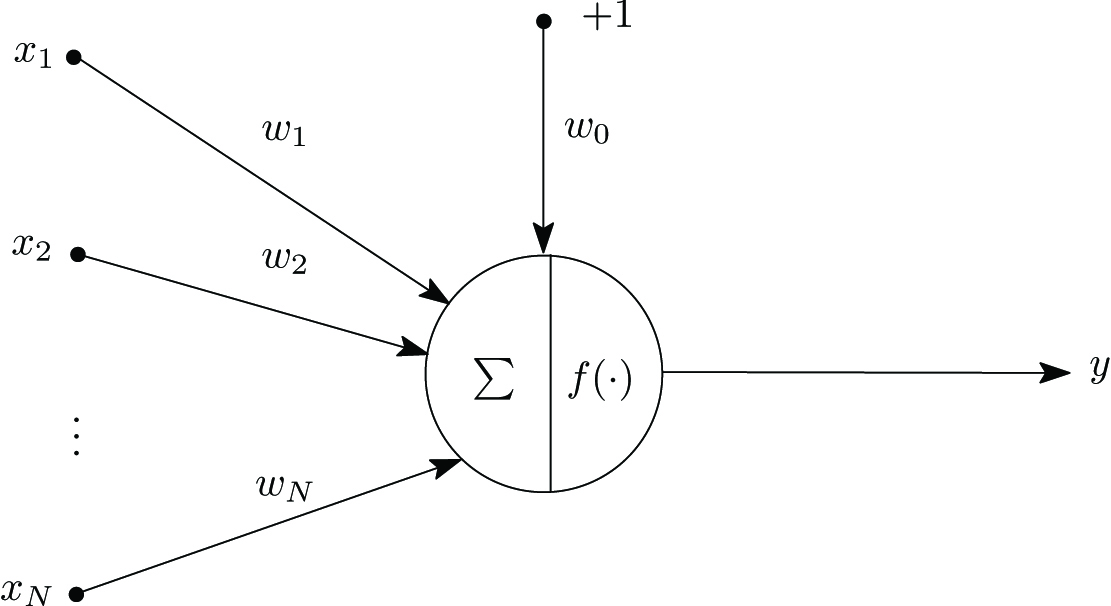
\includegraphics[width=0.6\textwidth]{./img/neuron}
\caption{Neurônio artificial: a combinação linear das entradas \emph{x} ponderadas pelos pesos \emph{w} é transformada pela função de ativação \emph{f} na saída \emph{y}.}
\label{img:neuronioArtificial}
\end{figure}

% Funções de ativação

A função $f$ é chamada de \emph{função de ativação} e fornece a resposta de um neurônio para uma dada entrada. Esta função precisa ser monotônica e contínua, podendo comumente ser as funções identidade, sigmóide, tangente hiperbólica, ou a retificada linear (ReLU) \cite{ref:JAI-2017}. Estas funções encontram-se representadas na Figura \ref{img:funcs_ativacao}.

\begin{figure}[h!]
	\centering
	\subfloat[Função identidade. \label{img:func_id}]{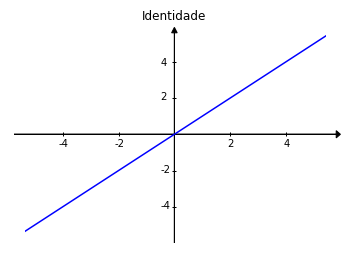
\includegraphics[width=0.4\linewidth]{./img/id}}
	\subfloat[Função sigmóide.\label{img:func_sigmoide}]{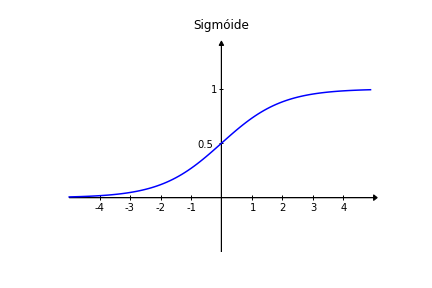
\includegraphics[width=0.4\linewidth]{./img/sigmoide}}\\
	\subfloat[Função tangente hiperbólica. \label{img:func_tanh}]{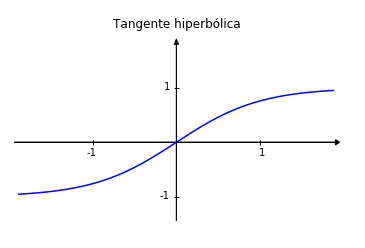
\includegraphics[width=0.4\linewidth]{./img/tanh}}
	\subfloat[Função retificada linear.\label{img:func_relu}]{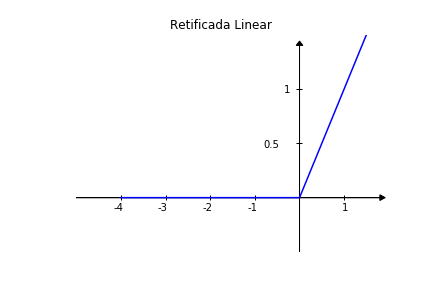
\includegraphics[width=0.4\linewidth]{./img/relu}}
	\label{img:funcs_ativacao}
	\caption{Exemplos de diferentes funções de ativação.}
	\label{img:funcs_ativacao}
\end{figure}

% Camadas ocultas

Neurônios artificiais individuais têm uma capacidade computacional limitada, independentemente da função de ativação escolhida, pois resolvem apenas problemas linearmente separáveis. No entanto, um conjunto de neurônios artificiais conectados na forma de uma rede -- \emph{rede neural artificial} -- adquirem a capacidade de resolver problemas de elevada complexidade \cite{ref:teresa}. A alternativa mais utilizada para resolver estes problemas é distribuir os neurônios em uma ou mais camadas conhecidas como  camadas ocultas \cite{ref:faceli}. Segundo Cybenko, uma rede com uma camada oculta pode implementar qualquer função contínua e uma rede com duas camadas ocultas permite a aproximação de qualquer função \cite{ref:cybenko}.

% Multilayer Perceptron

As RNAs do tipo Perceptron Multicamadas (MLP, do inglês \emph{Multilayer Perceptron}) apresentam uma camada de entrada, uma ou mais camadas ocultas e uma camada de saída. Uma das principais características de uma rede MLP é o seu alto grau de conectividade entre os neurônios, cuja intensidade está associada aos pesos da rede.

Cada neurônio em uma rede MLP atua ponderando as entradas recebidas dos neurônios de uma camada anterior a ele conectados, produzindo como saída um valor, resultante de sua função de ativação, que é propagado às camadas seguintes da rede neural. Conforme exemplificado na Figura \ref{img:rede-mlp}, a combinação das atuações individuais desempenhadas por cada neurônio da rede que define a atuação associada à RNA como um todo \cite{ref:teresa,ref:faceli,ref:haykin}.


\begin{figure}[h!]
	\centering
	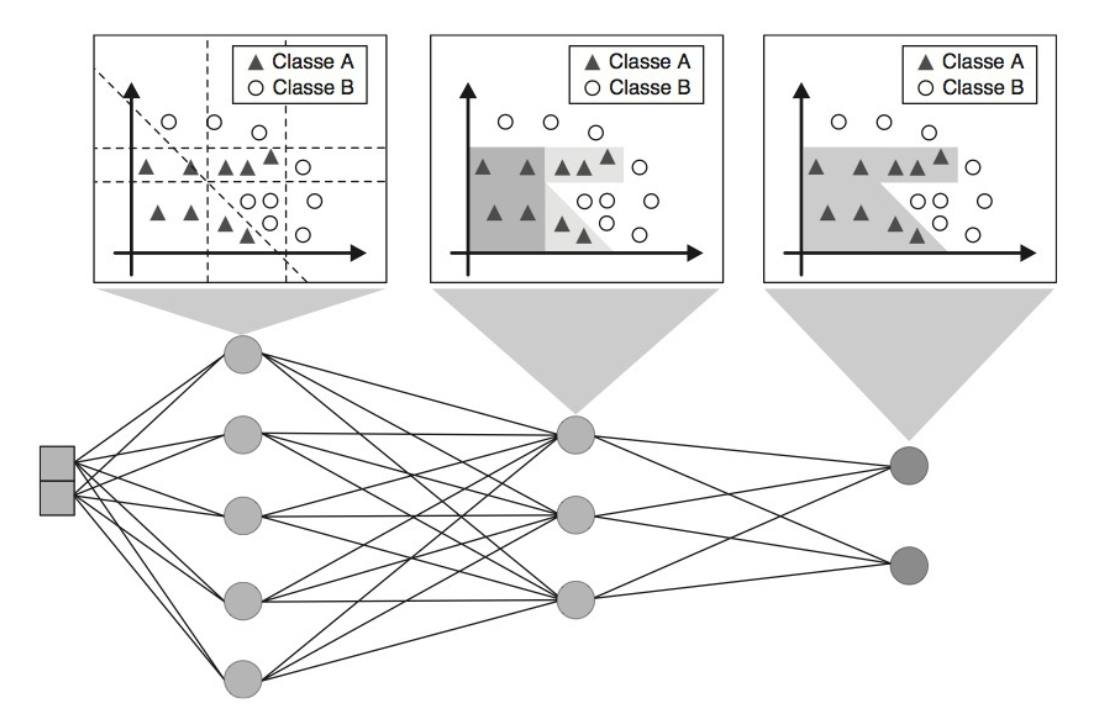
\includegraphics[width=1\textwidth]{./img/rede-mlp}
	\caption{Papel desempenhado pelos neurônios das diferentes camadas de uma rede MLP. Fonte: \cite{ref:faceli}.}
	\label{img:rede-mlp}
\end{figure}

% Aprendizado

Uma importante característica das RNAs é a sua capacidade de aprender por meio de exemplos. O processo de \emph{aprendizado} de uma rede neural consiste em sucessivos ajustes de pesos associados aos seus neurônios, de modo a aprimorar seu desempenho de acordo com um critério pré-estabelecido. Tais ajustes são realizados por algoritmos de treinamento formados por um conjunto de regras bem definidas que especificam quando e como deve ser alterado o valor de cada peso. Diversos algoritmos de aprendizado foram propostos, dentre os quais se destacam aqueles que seguem o paradigma de \emph{aprendizado supervisionado} \cite{ref:faceli,ref:patrick-tcc}.

% Paradigmas de aprendizado

O aprendizado supervisionado ajusta os pesos aplicando um conjunto de exemplos de treinamento rotulados. Cada exemplo consiste em um sinal de entrada associado à sua resposta alvo desejada. A cada padrão de entrada submetido à rede, compara-se a resposta desejada com a resposta calculada, ajustando-se os pesos das conexões para minimizar o erro \cite{ref:haykin}.

% Backpropagation

O algoritmo mais utilizado para o treinamento de redes MLP é o algoritmo \emph{backpropagation}, também chamado de retropropagação do erro ou ainda regra delta generalizada. Este algoritmo respeita o aprendizado supervisionado em que os pesos são modificados e ajustados para reduzir a distância entre a resposta desejada e a resposta produzida pela rede \cite{ref:haykin}. O treinamento é constituído da iteração de duas fases, uma fase para frente (\emph{forward}) e uma fase para trás (\emph{backwards}) \cite{ref:faceli}. A fase \emph{forward}, que compreende o fluxo da informação a partir da entrada até a saída da rede, é utilizada para produzir uma saída para um dado sinal de entrada. A fase \emph{backwards}, com fluxo da informação da saída da rede em direção à entrada, utiliza a diferença entre as saídas desejada e produzida para atualizar os pesos das conexões entre os neurônios e assim minimizar o erro \cite{ref:teresa}. Os ciclos de apresentação dos dados de treinamento e eventuais ajustes de pesos no \emph{backpropagation} são iterados até que seja atingido um critério de parada como, por exemplo, um número máximo de ciclos ou uma taxa máxima de erro \cite{ref:faceli}.


% Aplicações

As RNAs são modelos computacionais com ampla aplicação na resolução de problemas de previsão. Algumas aplicações utilizam RNAs para predição de condições climáticas, como em \cite{ref:apl-clima1} e \cite{ref:apl-clima2}, em que se deseja prever precipitações de chuva de determinados locais. Diversas outras aplicações de RNAs dizem respeito à classificação de padrões. Dentre as aplicações na área de classificação financeira, uma das mais bem sucedidas é a análise de crédito \cite{ref:teresa}. Além disso, as RNAs também são muito utilizadas para diagnósticos médicos, como em \cite{ref:apl-diagnostico1} e \cite{ref:apl-diagnostico2}. Outras aplicações tratam de reconhecimento de caracteres \cite{ref:apl-caracteres}, robótica \cite{ref:apl-robotica}, jogos \cite{ref:apl-jogos}, comunicação \cite{ref:meu-artigo}, dentre outros.

\subsection{\textit{Deep Learning}} \label{subsec:deep}
\emph{Deep Learning} (DL), ou Aprendizado Profundo, é uma subárea do AM especialmente baseada na utilização de RNAs com uma grande quantidade de camadas e neurônios para aprender padrões complexos em um vasto volume de dados \cite{ref:chollet,ref:khan,ref:gulli}. Por meio do reconhecimento de padrões, os modelos baseados em DL são capazes de reconhecer, traduzir, sintetizar e até prever padrões das mais diferentes naturezas \cite{ref:JAI-2017}.

As técnicas de DL têm sido aplicadas com êxito em muitos problemas, especialmente considerando dados de alta dimensionalidade, a exemplo de imagens e vídeos, e contextos em que há uma grande disponibilidade de exemplos  \cite{ref:JAI-2017,ref:khan}. Os modelos de DL têm se destacado, por exemplo, em muitas aplicações de saúde, especialmente considerando a detecção automática de padrões em imagens médicas para fins diagnósticos \cite{ref:yang}. O desafio
\emph{ImageNet Large Scale Visual Recognition Challenge}, de caráter anual realizado desde 2010, também têm promovido a proposição e competição de modelos de vanguada para fins de detecção de objetos e classificação de imagens em larga escala, contribuindo para o desenvolvimento do estado da arte em VC \cite{ref:image-net}.

Os modelos e técnicas de DL têm sido aplicados em tarefas de aprendizado supervisionado e não supervisionado, em que as redes neurais convolucionais têm sido o modelo mais proeminente. A seção a seguir apresenta o detalhamento deste modelo, suas características e conceitos associados.

\subsubsection{Redes Neurais Convolucionais} \label{subsec:cnn}
As \textit{Redes Neurais Convolucionais}, do inglês \textit{Convolutional Neural Networks} (CNNs), são modelos de redes neurais especializados em processamento de dados compostos pela união de vários segmentos elementares denominados camadas \cite{ref:goodfellow}. Cada camada possui uma finalidade específica e implementa uma determinada funcionalidade básica como convolução, normalização, \textit{pooling}, etc \cite{ref:khan}.

A camada convolucional é a camada mais importante de uma CNN e utiliza uma operação matemática linear chamada \textit{convolução} \cite{ref:goodfellow}. O processo de convolução é aplicado em um conjunto de \textit{filtros} e uma dada entrada para gerar uma saída conhecida como \textit{mapa de características}. Cada filtro consiste em uma matriz de números discretos que representam os pesos da CNN \cite{ref:khan}.

%cálculo da convolução


A camada convolucional recebe um volume de entrada de largura $w_{in}$, altura $h_{in}$ e profundidade $d_{in}$ e pode possuir um preenchimento  $p$ de zeros (\textit{zero-padding}), aplicado ao redor da entrada. Essa entrada é processada por $k$ filtros que representam os pesos e as conexões da CNN. Cada filtro possui uma extensão espacial $e$, que é igual ao valor da altura e da largura do filtro, e um \textit{stride} $s$, que é a distância entre as aplicações consecutivas do filtro no volume de entrada. A saída da camada de convolução é um volume de largura $w_{out}$ calculado conforme a Equação \ref{eq:wout}, altura $h_{out}$ conforme Equação \ref{eq:hout}  e profundidade $d_{out}$ igual a $k$ \cite{ref:buduma}. 

\begin{equation}
w_{out} = \frac{w_{in} - e + 2p}{s} +1 \label{eq:wout}
\end{equation}

\begin{equation}
h_{out} = \frac{h_{in} - e + 2p}{s} +1 \label{eq:hout}
\end{equation}

\subsubsection{Arquiteturas Canônicas de Redes Neurais Convolucionais} \label{subsubsec:arquiteturas}
Como mencionado anteriormente, o desafio anual \emph{ImageNet Large Scale Visual Recognition Challenge} (ILSVRC) têm tido um papel protagonista no desenvolvimento de soluções em DL, pois têm promovido um contexto para proposição e comparação de algumas das arquiteturas de CNNs mais bem sucedidas para problemas de detecção de objetos e classificação de imagens em larga escala \todo{Incluir citação}.

\todo{Uma figura da evolução da competição ano a ano? Quais as métricas? Qual o ganho? Mencionar um pouco mais a contribuição desta competição}

\todo{Como diz no site do ILSVRC: Citation
When reporting results of the challenges or using the datasets, please cite:
Olga Russakovsky*, Jia Deng*, Hao Su, Jonathan Krause, Sanjeev Satheesh, Sean Ma, Zhiheng Huang, Andrej Karpathy, Aditya Khosla, Michael Bernstein, Alexander C. Berg and Li Fei-Fei. (* = equal contribution) ImageNet Large Scale Visual Recognition Challenge. IJCV, 2015. paper | bibtex | paper content on arxiv | attribute annotations. Lá tem o bibtex. Trocar as referências ao longo do texto}

Embora os conceitos das camadas de uma CNN estejam bem estabelecidos e sejam de conhecimento geral, nem sempre é uma tarefa fácil propor uma rede neural deste tipo para um determinado cenário. Assim, uma consequência positiva da realização do ILSVRC é promover a difusão das arquiteturas de destaque na competição, as quais passam ser conhecidas e adaptadas pela comunidade acadêmica e tecnológica na resolução de diversos outros problemas. Considerando esta importância e potencial de aproveitamento de soluções, a seguir são apresentadas algumas destas arquiteturas canônicas.


\paragraph{LeNet} Yann le Cun desenvolveu, em 1990, uma das primeiras arquiteturas utilizadas para o reconhecimento de dígitos manuscritos, a LeNet. Vencedora do ILSVRC 2010, esta arquitetura é composta por três camadas convolucionais alternadas com camadas de \textit{pooling} seguidas de duas FCLs conforme representado na Figura \ref{img:lenet} \cite{ref:sewak,ref:khan}.

\begin{figure}[!ht]
	\centering
	\caption{Arquitetura LeNet de CNN. Fonte: \cite{ref:khan}.}
	\label{img:lenet}
	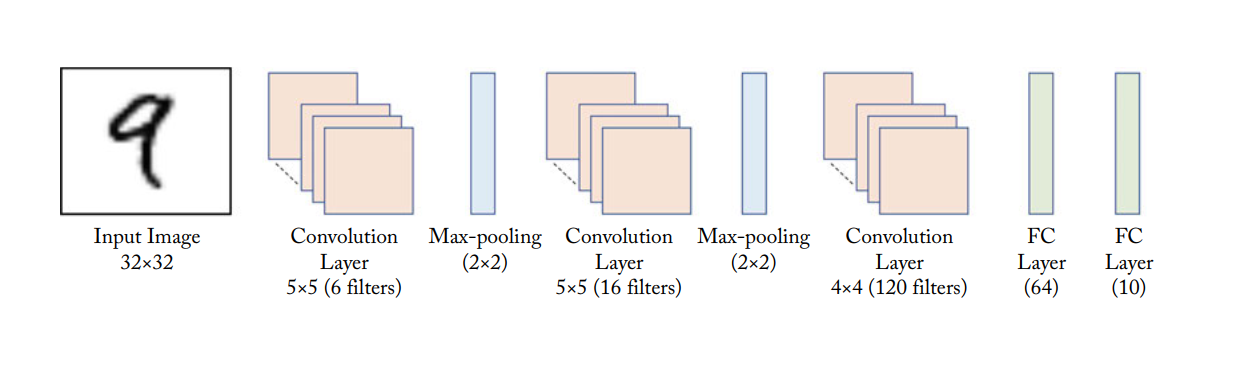
\includegraphics[width=1\textwidth]{./img/lenet}
\end{figure}


\paragraph{AlexNet} Em 2012, a vencedora do ILSVRC foi a arquitetura proposta por Alex Krizhevsky, conhecida como AlexNet, ilustrada na Figura \ref{img:alexnet}. A AlexNet é mais profunda e uma versão muito mais ampla da arquitetura LeNet \cite{ref:satapathy}. A principal diferença entre a AlexNet e as CNNs predecessoras é a sua maior profundidade, que lida muito bem com sua grande quantidade de parâmetros, além da utilização de artifícios como \textit{dropout} e \textit{data augmentation}. As cinco primeiras camadas da arquitetura AlexNet são camadas de convolução e \textit{pooling} alternadas de forma similar à LeNet, porém, seguem-se mais duas camadas uma convolucional e uma de\textit{pooling}. As três últimas camadas são FCL, mas além destas existem camadas \textit{dropout} que ajudam à reduzir \textit{overfiting} \cite{ref:khan}. \todo{Acho que a citação para alexnet está errada.}

\begin{figure}[!ht]
	\centering
	\caption{Arquitetura da AlexNet. Fonte: \cite{ref:khan}.}
	\label{img:alexnet}
	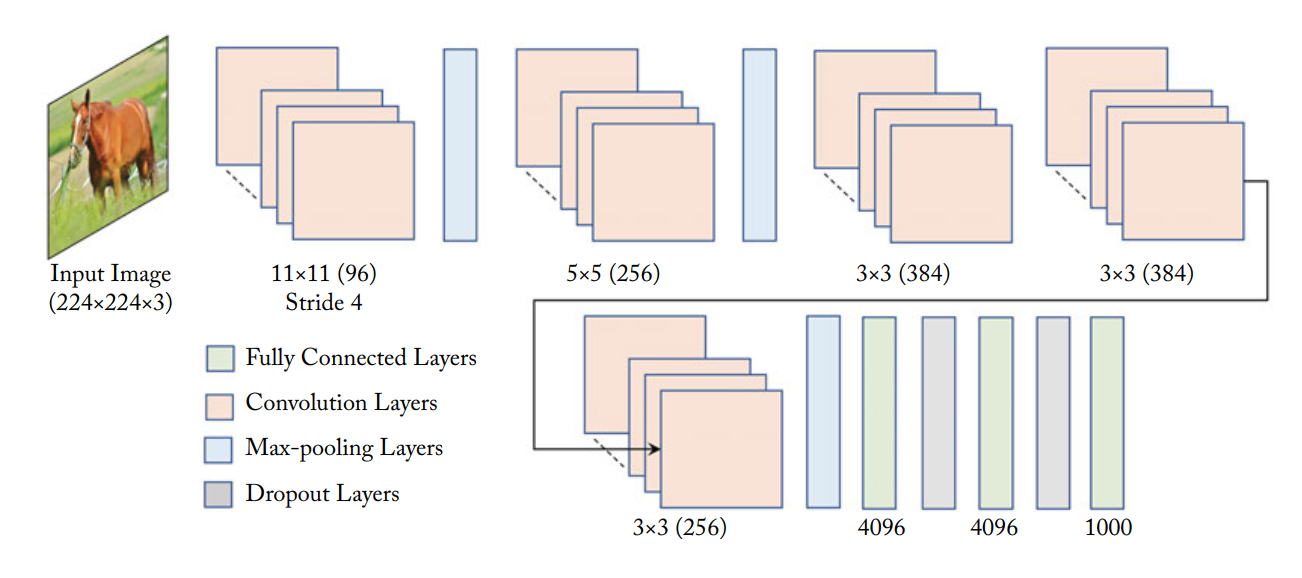
\includegraphics[width=1\textwidth]{./img/alexnet}
\end{figure}

\paragraph{VGGNet} A arquitetura VGGNet é uma das arquiteturas mais populares desde sua criação em 2014, apesar de não ter sido a vencedora do ILSVRC realizado no respectivo ano. A razão de sua popularidade se dá especialmente em virtude do uso de pequenos filtros de convolução, diminuindo o número de parâmetros ajustáveis e, por conseguinte, aumentando a eficiência do treinamento. A arquitetura VGGNet usa estritamente fitros de convolução de dimensão $3 \times 3$ combinados com camadas de \textit{pooling} para extração de características e um conjunto de três FCLs. Além das camadas de convolução, \textit{pooling} e das camadas conectadas, esta arquitetura também possui as camadas \textit{dropout} como pode ser observado na Figura \ref{img:vggnet} \cite{ref:khan}.

\begin{figure}[!ht]
	\centering
	\caption{Arquitetura VGGNet. Fonte: \cite{ref:khan}.}
	\label{img:vggnet}
	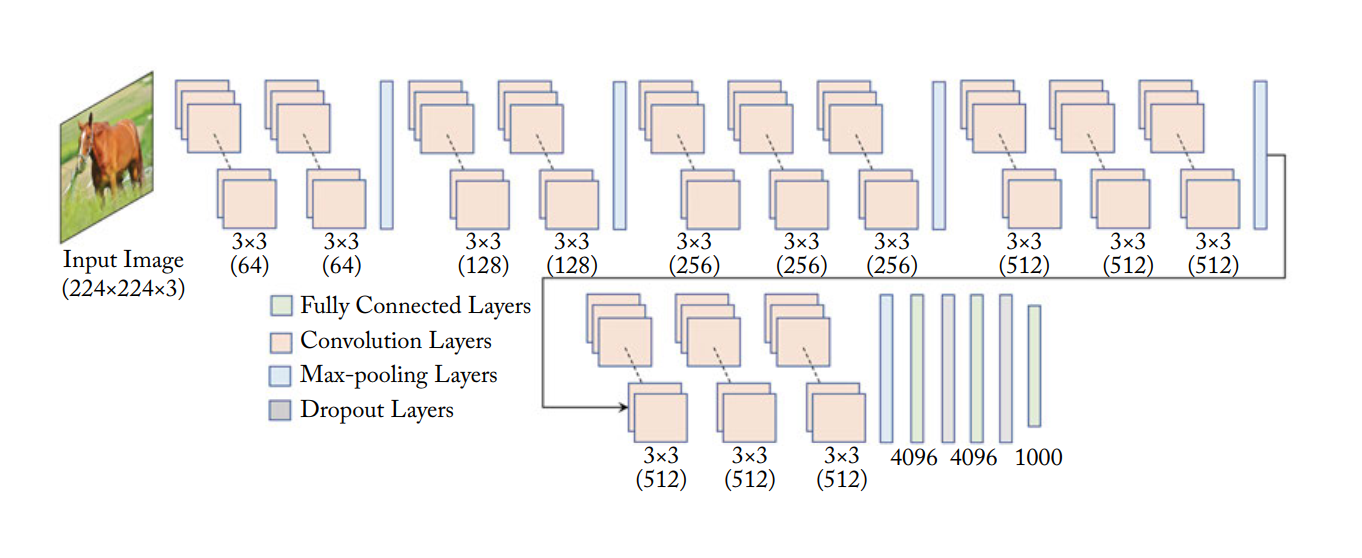
\includegraphics[width=1\textwidth]{./img/vggnet}

\end{figure}

\paragraph{GoogLeNet} Desenvolvida pela empresa Google e vencedora do ILSVRC 2014, a arquitetura GoogLeNet possui $22$ camadas baseadas em um módulo elementar chamado \emph{Inception Module}. O processamento desses módulos ocorre de forma paralela, diferentemente do processamento sequencial das arquiteturas discutidas anteriormente. A ideia central da arquitetura GoogLeNet é paralelizar os módulos e combinar as características da saída sem se preocupar com as funções individuais de cada camada. No entanto, essa abordagem resulta em um mapa de características com muitos elementos, mas para contornar este problema, após a execução do primeiro módulo, a rede realiza uma redução de dimensionalidade utilizando uma FCL antes de continuar o processo de treinamento \cite{ref:khan}. A representação da arquitetura GoogLeNet encontra-se na Figura \ref{img:googlenet}.

\begin{figure}[!ht]
	\centering
	\caption{Arquitetura GoogLeNet. Fonte: \cite{ref:khan}.}
	\label{img:googlenet}
	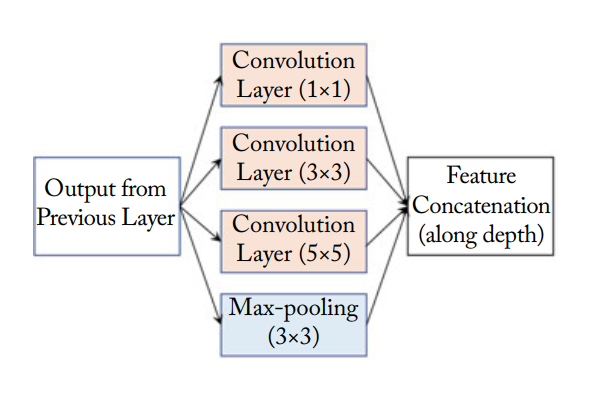
\includegraphics[width=0.6\textwidth]{./img/googlenet}

\end{figure}


\subsection{\textit{Transfer Learning}} \label{subsec:transfer}
\emph{Transfer Learning} (TL), ou Transferência de Conhecimento, é uma poderosa técnica de DL a qual possui diversas aplicações em diferentes domínios \cite{ref:gulli}. Ao invés de estruturar uma arquitetura de uma CNN e treiná-la por completo, esta técnica permite reutilizar uma rede pré-treinada e adaptá-la a um novo conjunto de dados \cite{ref:sewak}. Modelos que foram pré-treinados utilizando um vasto e genérico conjunto de dados conseguem capturar características universais, como por exemplo curvas e arestas, em suas primeiras camadas \cite{ref:zaccone}.

As técnicas de TL podem ser utilizadas de diferentes maneiras, baseando-se nas arquiteturas das CNNs. Existem alguns modelos disponíveis para aplicações que foram pré-treinados utilizando as principais arquiteturas canônicas de CNN e aprenderam as características de grandes conjuntos de dados bastante conhecidos, como o ImageNet e o Places205 \cite{ref:image-net,ref:places205}. Para diferentes tarefas, esses modelos podem ser alterados modificando a camada de saída e fazendo um retreinamento nas últimas camadas das redes para se obter o aprendizado desejado \cite{ref:khan}. 


\subsection{Espaço de Cores CIELab} \label{subsec:cores}
Um espaço de cores é um modelo matemático utilizado para descrever uma determinada cor representando um \emph{gamut}, isto é, uma paleta de cores que uma certa tecnologia é capaz de reproduzir. Existem diversos modelos de espaços de cores, tais como RGB e CIELab, os quais possuem diferentes  formas de representação \cite{ref:galleti}.

A sigla RGB é uma abreviatura de um espaço de cores formado por três canais: um R, que vem do inglês \emph{red} (vermelho); outro G, do inglês \emph{green} (verde); e o outro B, do inglês \emph{blue} (azul). O RGB forma a síntese aditiva em que, pela sobreposição das três luzes em um ambiente totalmente escuro, obtém-se a luz branca, como ilustrado na Figura \ref{fig:rgb}. Em cada um dos três canais deste espaço de cores, um valor de intensidade é atribuído para cada \emph{pixel} de uma imagem, variando de $0$ a $255$. Essa atribuição tem como finalidade a composição de uma imagem colorida e é muito utilizada na indústria gráfica digital e em mídias digitais, como televisão, câmeras, escâneres, \emph{smartphones}, etc \cite{ref:galleti}.

\begin{figure}[h!]
	\centering
	\caption{Síntese aditiva do espaço de cores RGB. Fonte: \cite{ref:galleti}.}
	\label{fig:rgb}
	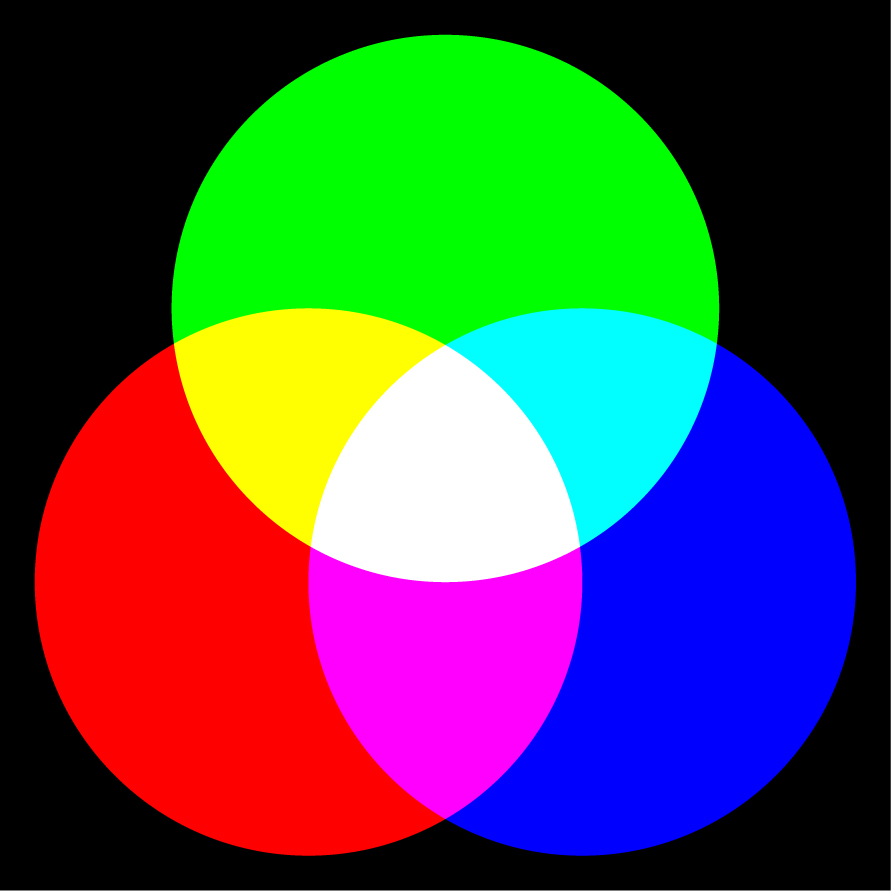
\includegraphics[width=0.3\textwidth]{./img/rgb}
\end{figure}


A \emph{Commision Internationale L'Eclairage} (CIE), deu nome a um outro espaço de cores bastante utilizado como referência para gerenciamento de cores no tratamento de imagens, o CIELab. A sigla Lab retrata os três canais utilizados por esse sistema os quais estão graficamente representados na Figura \ref{fig:cielab}. O canal simbolizado pela letra $L$ indica luminosidade, variando de preto a branco e os canais das letras $a$ e $b$ são os eixos de cromaticidade, em que $a$ varia de vermelho a verde e $b$ varia de azul a amarelo. Nesse modelo, a separação de cores é feita de maneira a deixar um canal responsável pela formação do desenho da imagem (canal $L$), e os outros dois canais ($a$ e $b$) ficam responsáveis apenas pelas informações das cores \cite{ref:galleti}.

\begin{figure}[h]
	\centering
	\caption{Representação gráfica do espaço de cores CIELab. Fonte: \cite{ref:galleti}.}
	\label{fig:cielab}
	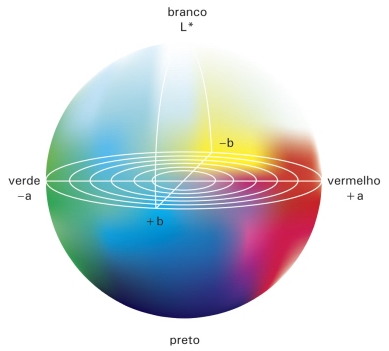
\includegraphics[width=0.4\textwidth]{./img/cielab}
\end{figure}


\subsection{Tecnologias Utilizadas} \label{subsec:tecnologias}
As tecnologias e bibliotecas predominantemente utilizadas neste trabalho envolvem e s�o compat�veis com a linguagem de programa��o Python, pois esta tem se destacado amplamente em projetos de AM em diversos cen�rios. Esta � uma linguagem de programa��o interpretada, interativa, multi-paradigma,  de alto n�vel, multi-plataforma, com uma sintaxe simples e c�digo aberto, idealizada por Guido van Rossum no in�cio da d�cada de 1990 \cite{ref:python}.

Para o processamento das imagens em termos de redimensionamento, persist�ncia, mudan�a e consulta do espa�o de cores, as bibliotecas \texttt{PIL} (Pillow) e \texttt{colormath} tiveram um papel protagonista \cite{lib:pillow,lib:colormath}. No tocante � manipula��o de arquivos, contemplando abertura, leitura e busca por extens�es similares, as bibliotecas \texttt{os} e \texttt{glob} foram utilizadas \cite{lib:os,lib:glob}. A manipula��o do conjunto de imagens e de suas respectivas representa��es matriciais ficou por conta da \texttt{numpy}, uma biblioteca fundamental para computa��o cient�fica que � extremamente poderosa para gerenciamento e altera��es de matrizes de muitas dimens�es \cite{lib:numpy}.  Ademais, no que diz a respeito do treinamento e testes dos modelos de AM, as bibliotecas \texttt{scikit-learn} e \texttt{keras} foram consideradas, em que a primeira teve um papel principal nos c�lculos autom�ticos das m�tricas de desempenho e a segunda nos modelos de DL com par�metros previamente configurados \cite{lib:scikit,lib:keras}.

Por fim, a infra-estrutura de computa��o em nuvem provida pelo Google Cloud Platform (GCP) totalmente voltada para projetos de AM foi essencial para o desenvolvimento deste projeto. As m�quinas virtuais oferecidas pela plataforma aumentaram o poder computacional acess�vel possibilitando um processamento mais favor�vel ao cen�rio em quest�o. A manipula��o e pr�-processamento do conjunto �ntegro de imagens, o treinamento dos modelos de DL e a fase de an�lise desses modelos foram executados em inst�ncias dispon�veis pelo GCP tendo em vista os recursos de mem�ria e processamento necess�rios \cite{tec:gcloud}.



\section{Trabalhos Relacionados} \label{sec:relacionados}
Diversos trabalhos na literatura têm abordado o tema de colorização de imagens, como \cite{ref:rel-zhang} \todo{incluir aqui mais duas citações de trabalhos relacionados}. Esta seção apresenta as técnicas utilizadas por \cite{ref:rel-zhang} para o problema de colorização, as quais dispõem conceitos de ML e DL.

Zhang propõe uma abordagem totalmente automatizada que produz colorizações vibrantes e realistas utilizando CNNs \emph{feedfoward} treinadas com milhões de imagens. No trabalho em questão, o canal de luminosidade $L$ é apresentado a modelos que preveem os canais de cromaticidade $a$ e $b$ correspondentes de uma imagem no espaço de cores CIELab. No entanto, os autores ressaltam que este cenário produz imagens coloridas com baixa saturação. Considerando a colorização de um domínio multimodal, uma das explicações citadas para este problema são as métricas utilizadas que podem estimular previsões conservadoras.
 
Para contornar este problema, os autores adotaram algumas técnicas matemáticas que favorecem problemas multimodais realizando re-treinamentos para enfatizar as cores menos frequentemente utilizadas. Esta abordagem explora a diversidade do conjunto de dados e propõe resultados com cores mais vibrantes e perceptivamente mais realistas.

O principal objetivo do trabalho de Zhang era obter resultados visualmente agradáveis para o ser humano. Deste modo, os autores desenvolveram um método próprio de avaliação intitulado ``Colorization Turing Test'' (CTT). Este método apresentava aos avaliadores uma imagem colorida e a imagem correspondente colorida pelas redes neurais propostas e solicitava a identificação da imagem real. Os CTTs confundiram $32\%$ dos dos avaliadores, um resultado significativamente maior que outros trabalhos similares da literatura.

Alguns aspectos do trabalho de Zhang foram relevantes para o contexto deste trabalho. Um desses aspectos foi a estruturação dos atributos utilizados para o treinamento das CNNs. Considerando uma imagem no espaço de cores CIELab, a entrada dos modelos propostos será a luminosidade $L$ de uma dada imagem para obtenção das colorações $a$ e $b$ correspondentes. No entanto, devido a limitação de recursos computacionais, as técnicas utilizadas considerando o cenário multimodal não serão abordadas.

Sabendo que os recursos computacionais disponíveis são escassos, a solução encontrada para aprimorar o treinamento das redes neurais convolucionais foi a utilização das técnicas de TL, as quais utilizam modelos pré-treinados com grandes conjuntos de dados para extração de características. Essas técnicas disponibilizam os pesos ajustados durante o treinamento dos modelos como uma forma de transferência de conhecimento para agregar aprendizagem aos modelos adaptados ao cenário em questão.  


\section{Solução Proposta} \label{sec:solucao}
\subsection{Visão Geral da solução proposta} \label{sec:visaogeral}
\subsubsection{Tarefa de Aprendizado} \label{subsubsec:tarefa}
No contexto deste trabalho, o problema da colorização de uma imagem será abordado como uma \emph{tarefa de regressão}, cujo objetivo é obter uma estimativa dos parâmetros de coloração dos pixels. De maneira mais detalhada, a Figura \ref{fig:aprendizado} ilustra o conjunto de passos a ser realizado.

\begin{figure}[h]
	\centering
	\caption{Detalhamento do processo de aprendizado.}
	\label{fig:aprendizado}
	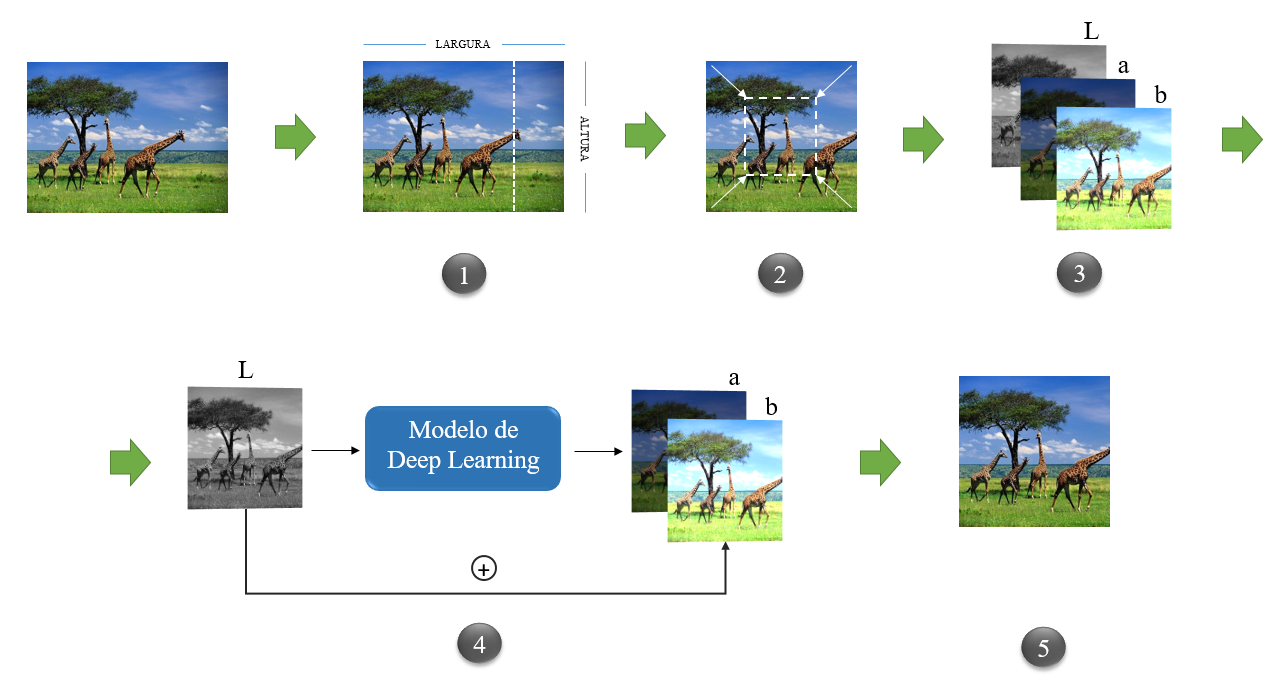
\includegraphics[width=0.95\textwidth]{./img/aprendizado}
\end{figure}

Dada uma imagem em tons de cinza que se deseja colorir, o primeiro passo a ser realizado (Passo 1) consiste no redimensionamento da imagem de acordo com a dimensão predominante (altura ou largura), com vistas a obter uma imagem quadrada. Em seguida, para que seja fornecida como entrada para os modelos de DL, a imagem será redimensionada para $128 \times 128$ pixels (Passo 2). Após esta etapa, o espaço de cores da imagem será convertido de RGB para CIELab (Passo 3). Desta conversão, o parâmetro de luminosidade $L$ será fornecido para o modelo de DL, cujo objetivo será produzir duas matrizes com os valores de coloração $a$ e $b$ (Passo 4). Por fim, a luminosidade $L$, já conhecida, será combinada com as matrizes de coloração $a$ e $b$ produzidas, compondo uma versão colorida da imagem inicial (Passo 5).

Para que os modelos propostos para realização da coloração produzam resultados factíveis, é necessária uma etapa de treinamento, em que imagens coloridas serão fornecidas sucessivamente às redes para ajustes dos pesos, produzindo mapas de características mais fidedignos ao domínio do problema. A base de dados a ser utilizada para esta etapa será descrita na seção a seguir.

No escopo deste trabalho serão consideradas as arquiteturas canônicas de CNNs VGGNet  e ResNet as quais serão ajustadas ao problema em questão mediante TL. Diferentes valores de parâmetros e hiperparâmetros (épocas, taxa de aprendizado, \emph{batch size}, etc.) serão considerados, sempre que possível, buscando um melhor ajuste do modelo ao problema em questão.

Nesta tarefa de regressão, realizada de acordo com o paradigma supervisionado, a métrica de desempenho utilizada será o Erro Quadrático Médio (MSE, do inglês \emph{Mean Squared Error}), definido como:

\begin{equation}
\textrm{MSE} = \frac{1}{n}\sum_{i=1}^n (y_i - \hat{y}_i)^{2}, \label{eq:mse}
\end{equation} em que $y_i$ é o valor real esperado para o exemplo $i$, $\hat{y}_i$ é o valor previsto pelo modelo para este exemplo e $n$ é o número de amostras presentes no conjunto de dados \cite{ref:faceli}.

O treinamento e testes das CNNs seguirão a abordagem \emph{Holdout} de validação cruzada, em que $70\%$ dos dados serão utilizados no treino e ajuste de parâmetros e o restante para avaliação, com vista a capturar a qualidade da generalização proposta pelos modelos considerados \cite{ref:brink}.


\subsubsection{Dados Experimentais} \label{subsubsec:dados}
Para alcançar os objetivos propostos no escopo deste trabalho de conclusão de curso, a base de dados a ser utilizada no processo de aprendizado será o conjunto de validação da tarefa \emph{Fine-grained classification} do ILSVRC $2012$ que está disponível em \cite{ref:image-net}. A Figura \ref{fig:visaogeral} apresenta uma visão geral deste conjunto de dados que dispõe de um total de $50$ mil imagens de diferentes naturezas, as quais foram coletadas do \emph{website} Flickr e de outras plataformas semelhantes e rotuladas manualmente por ausência ou presença de $1000$ diferentes categorias \cite{ILSVRC}. 

\begin{figure}[h]
	\centering
	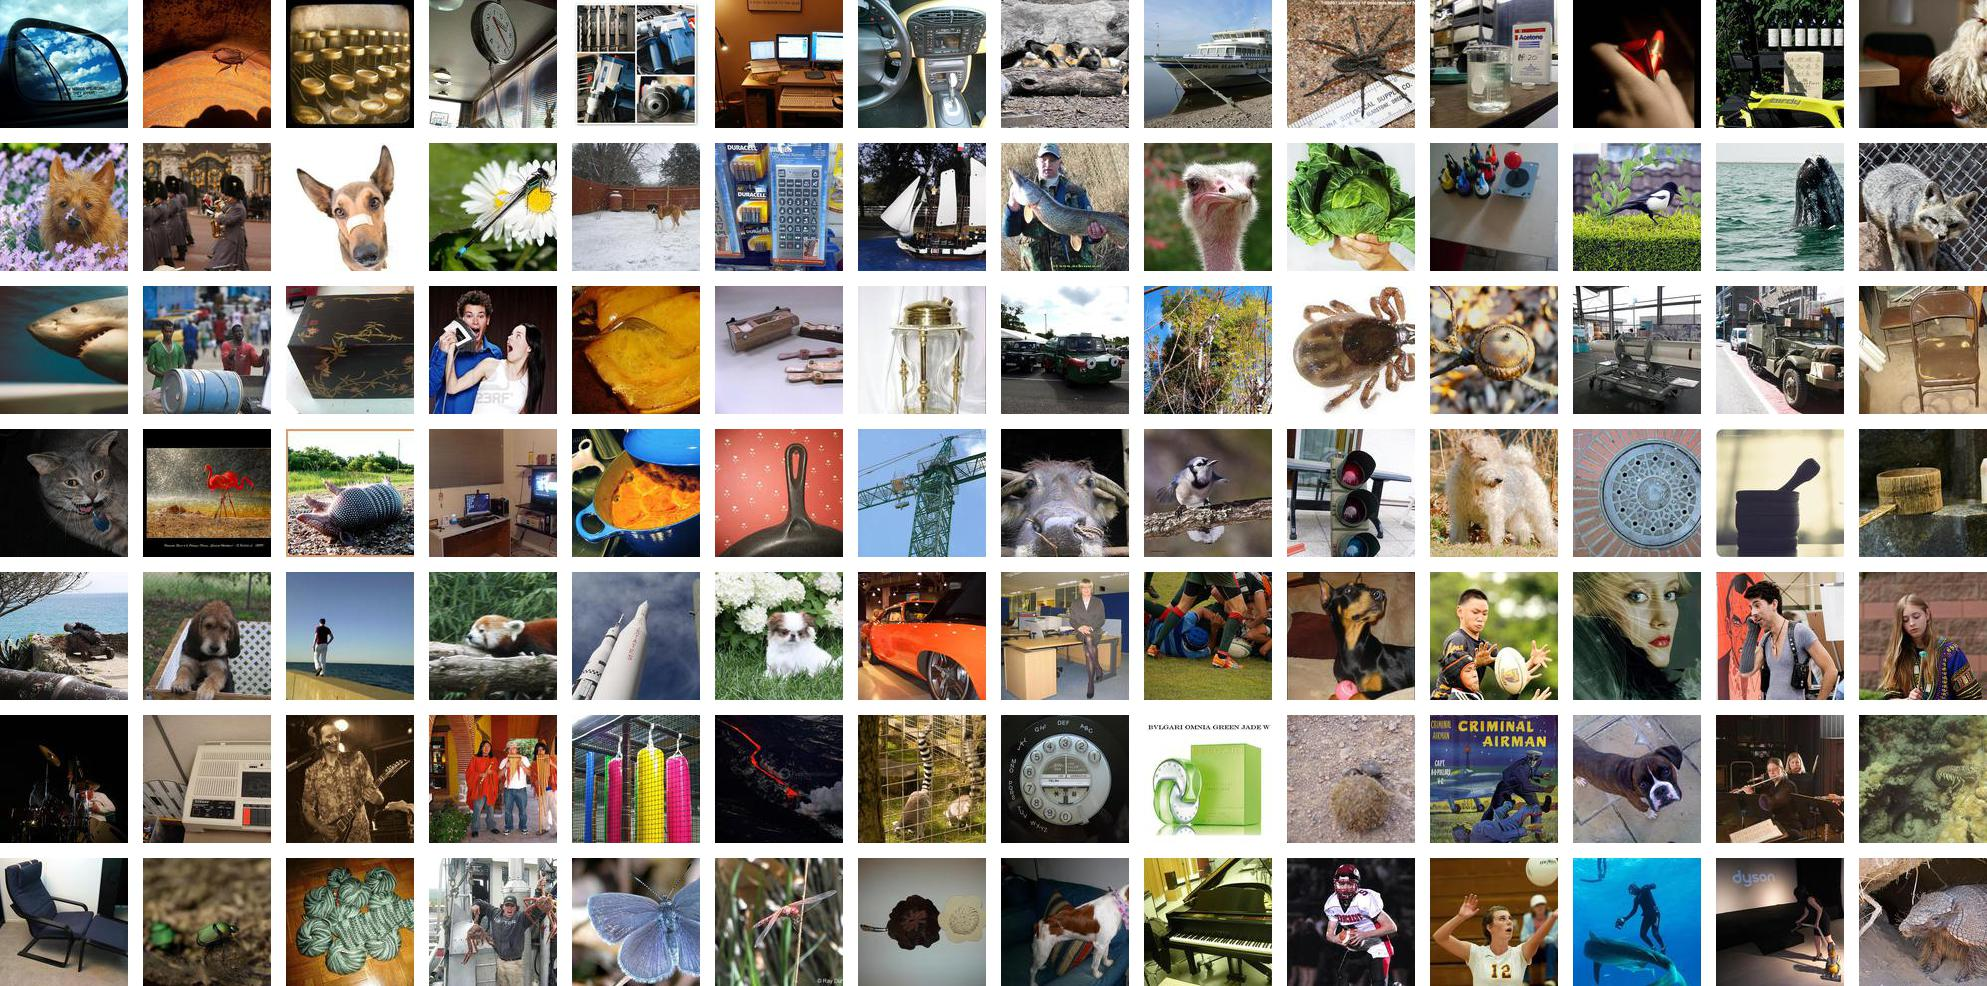
\includegraphics[width=1\textwidth]{./img/visaogeral}
	\caption{Visão geral do conjunto de dados.}
	\label{fig:visaogeral}
\end{figure}

Como dito anteriormente, conjunto de dados será particionado para compor o processo de aprendizado e desse modo $35$ mil imagens serão utilizadas para o treinamento e ajustes dos modelos e as outras $15$ mil para as análises de desempenho. Entretanto, antes de disponibilizar a base de dados para os modelos de DL, as imagens devem estar bem estruturadas e, portanto, devem passar por um pré-processamento, o qual será detalhado na Seção \ref{subsec:pre-process}.



\subsubsection{Limpeza e pré-processamento} \label{subsubsec:pre-process}
Como se sabe, algoritmos de AM precisam de quantidades significativas de dados que estejam preferencialmente sem muitos ruídos. Entretanto, com o aumento do tamanho do conjunto de dados os custos computacionais também aumentam e faz-se necessário um pré-processamento desses dados para estruturá-los da maneira ideal sem que haja uma excessiva sobrecarga computacional \cite{ref:marsland}.

O conjunto de imagens que será utilizado no processo de colorização deste trabalho será submetido a um pré-processamento que se inicia padronizando a dimensão das imagens. Primeiramente, as imagens são redimensionadas de forma que possuam os mesmos tamanhos de largura e altura, para obtenção de uma imagem quadrada. Em seguida, cada imagem é redimensionada para $128 \times 128$ pixels, padronizando todas as imagens nesta mesma dimensão. Esta padronização visa tornar a tarefa de aprendizado factível diante dos recursos computacionais disponíveis.

Após a etapa de redimensionamento, a etapa seguinte consistiu em selecionar as imagens cujo espaço de cores fosse o RGB. Isto foi efetuado com o intuito de eliminar imagens em tons de cinza e em outros espaços de cores que demandassem um maior processamento posterior. No caso das imagens em tons de cinza, em particular, a eliminação das mesmas simplifica o processo de treinamento dos modelos, visto que estas não fornecem informação relevantes para aprendizado de colorações. Nesta etapa, foram eliminadas cerca de $900$ imagens que se encaixam em um dos critérios mencionados.

Em seguida, todas as imagens foram então convertidas do espaço de cores RGB para o espaço de cores CIELab, tendo em vista a diminuição dos parâmetros de entrada e saída no processo de aprendizagem e também a adequação aos procedimentos descritos na Seção \ref{subsec:tarefa}. Cada imagem passou então a corresponder a uma matriz de dimensões $3\times 128 \times 128$, a qual foi separada em duas partes: componente $L$, de dimensões $128 \times 128$, a ser fornecida como \emph{entrada} para os modelos, e componentes $a$ e $b$, a serem fornecidos como rótulo de \emph{saída} para o aprendizado supervisionado dos modelos, com dimensões $2 \times 128 \times 128$.


\subsection{Análise Comparativa} \label{sec:analise}
\input{./files/solucao/analise}




\section{Considerações Parciais} \label{sec:consideracoes}
\begin{frame}{Considera��es Finais}
\begin{itemize}
\item \alert{Implementa��o} de aut�matos celulares bidimensionais
\begin{itemize}
\item Regra geral, total�sticos e total�sticos externos
\end{itemize}
\ \ \newline
\item Remodelagem da \alert{interface gr�fica} para a ferramenta CABuilder
\begin{itemize}
\item Utiliza��o da biblioteca PyQt
\item Funcionalidades preservadas
\item Fluxo de intera��o com o usu�rio mais simples e intuitivo
\item Acr�scimo da gera��o de aut�matos em forma de anima��o
\end{itemize}
\ \ \newline
\item \alert{An�lise estat�stica} das sequ�ncias produzidas pelos aut�matos celulares bidimensionais
\ \newline
\item CABuilder dispon�vel no reposit�rio: \url{http://goo.gl/wLE1jk}
\ \ \newline
\ \ \newline
\end{itemize}
\end{frame}


% Documentação abntex2cite
%http://mirrors.ibiblio.org/CTAN/macros/latex/contrib/abntex2/doc/abntex2cite.pdf
\bibliography{sbc-template}

\end{document}
